\documentclass[12pt,a4paper]{report}
\usepackage[margin=1in]{geometry}
\usepackage{graphicx}
\usepackage{amsmath,amssymb}
\usepackage{booktabs}
\usepackage{enumitem}
\usepackage{setspace}
\usepackage{titlesec}
\usepackage[hidelinks]{hyperref}
\usepackage{fancyhdr}
\usepackage{float}
\usepackage{caption}
\usepackage{times}

\onehalfspacing

% Chapter formatting
\titleformat{\chapter}[display]
  {\normalfont\Large\bfseries\centering}
  {Chapter \thechapter}{12pt}{\LARGE}
\titlespacing*{\chapter}{0pt}{-20pt}{20pt}

% Header/footer
\pagestyle{fancy}
\fancyhf{}
\fancyhead[R]{\thepage}
\renewcommand{\headrulewidth}{0.4pt}

\begin{document}

% ===========================================================================
% COVER PAGE
% ===========================================================================
\begin{titlepage}
\begin{center}

\vspace*{1cm}
{\large \textbf{A PROJECT REPORT}}\\[0.5cm]
{\large ON}\\[1cm]

{\LARGE \textbf{HYDRA-LB: An LSTM-Based Proactive Load Balancing\\Framework for Multi-Controller Software-Defined Networks}}\\[2cm]

{\large Submitted to}\\[0.3cm]
{\large \textbf{KIIT Deemed to be University}}\\[1.5cm]

{\large In Partial Fulfilment of the Requirement for the Award of}\\[0.5cm]
{\large \textbf{BACHELOR'S DEGREE IN}}\\[0.3cm]
{\large \textbf{INFORMATION TECHNOLOGY}}\\[1cm]

{\large BY}\\[0.5cm]
{\large YOUR NAME AND AFFILIATION}\\[2cm]

\vfill

{\large \textbf{SCHOOL OF COMPUTER ENGINEERING}}\\[0.3cm]
{\large \textbf{KALINGA INSTITUTE OF INDUSTRIAL TECHNOLOGY}}\\[0.3cm]
{\large \textbf{BHUBANESWAR, ODISHA -- 751024}}\\[0.3cm]
{\large April 2025}

\end{center}
\end{titlepage}

% ===========================================================================
% CERTIFICATE PAGE
% ===========================================================================
\newpage
\thispagestyle{empty}
\begin{center}
{\large \textbf{KIIT Deemed to be University}}\\[0.3cm]
{\normalsize School of Computer Engineering\\Bhubaneswar, ODISHA 751024}\\[2cm]

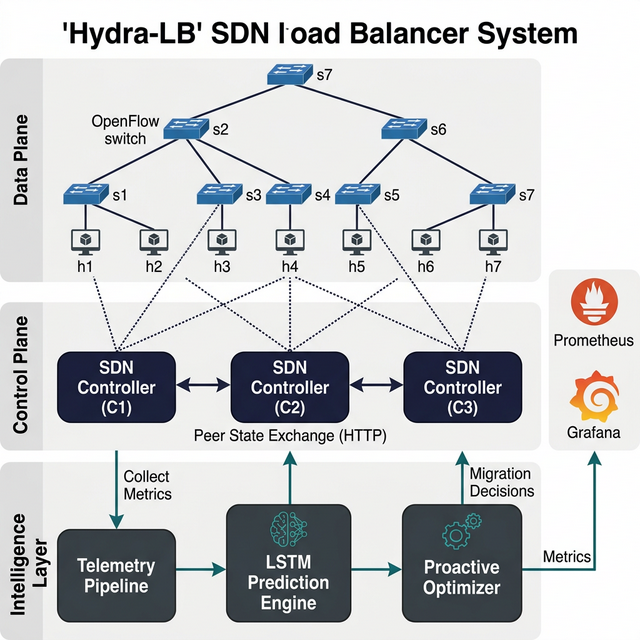
\includegraphics[width=2.5cm]{figures/system_architecture.png}\\[1cm] % Replace with university logo if available

{\LARGE \textbf{CERTIFICATE}}\\[1cm]
\end{center}

This is to certify that the project entitled

\begin{center}
\textbf{``HYDRA-LB: An LSTM-Based Proactive Load Balancing Framework for Multi-Controller Software-Defined Networks''}
\end{center}

\noindent submitted by

\begin{center}
\textbf{[Student Name 1, Roll No.]}\\
\textbf{[Student Name 2, Roll No.]}\\
\textbf{[Student Name 3, Roll No.]}\\
\textbf{[Student Name 4, Roll No.]}\\
\textbf{[Student Name 5, Roll No.]}\\
\textbf{[Student Name 6, Roll No.]}\\
\end{center}

\noindent is a record of bonafide work carried out by them, in the partial fulfilment of the requirement for the award of Degree of Bachelor of Engineering (Information Technology) at KIIT Deemed to be University, Bhubaneswar. This work is done during year 2024--2025, under our guidance.

\vspace{2cm}
\noindent Date:\hspace{0.5cm}/\hspace{0.5cm}/

\vspace{2cm}
\begin{flushright}
(Dr. ANJAN BANDYOPADHYAY)\\
Project Guide
\end{flushright}

% ===========================================================================
% ACKNOWLEDGEMENTS
% ===========================================================================
\newpage
\thispagestyle{empty}
\chapter*{Acknowledgements}
\addcontentsline{toc}{chapter}{Acknowledgements}

We are profoundly grateful to \textbf{Dr. ANJAN BANDYOPADHYAY} of \textbf{KIIT University} for his expert guidance and continuous encouragement throughout to see that this project reaches its target since its commencement to its completion.

We would also like to express our sincere thanks to the School of Computer Engineering for providing the necessary infrastructure and computational resources that made this research project possible.

\vspace{1cm}
\noindent \textbf{[Student Name 1]}\\
\textbf{[Student Name 2]}\\
\textbf{[Student Name 3]}\\
\textbf{[Student Name 4]}\\
\textbf{[Student Name 5]}\\
\textbf{[Student Name 6]}

% ===========================================================================
% ABSTRACT
% ===========================================================================
\newpage
\chapter*{Abstract}
\addcontentsline{toc}{chapter}{Abstract}

Multi-controller Software-Defined Networking (SDN) architectures are increasingly deployed to address the scalability limitations of centralized control planes. However, distributing network switches across controllers introduces a dynamic load balancing challenge: as traffic patterns shift, controllers become unevenly loaded, leading to elevated tail latency and reduced throughput. Existing approaches predominantly employ reactive strategies---such as round robin and least connections---that redistribute load only after imbalance has materialized.

In this project, we present HYDRA-LB, a proactive load balancing framework that leverages a bidirectional Long Short-Term Memory (LSTM) network augmented with temporal attention to forecast per-controller load three to five seconds into the future. A variance-aware optimization engine consumes these predictions and triggers preemptive switch migrations via OpenFlow role changes before congestion occurs. We implement HYDRA-LB on the Ryu SDN framework and evaluate it on emulated Fat-Tree data center topologies under four distinct traffic workloads---steady, burst, flash crowd, and skewed---using Mininet with Open vSwitch.

Experimental results demonstrate that HYDRA-LB reduces inter-controller load variance by up to 51.2\% compared to round robin and 34.8\% compared to least-load baselines, while maintaining comparable throughput and incurring negligible migration overhead. Our findings validate that LSTM-driven proactive optimization constitutes a viable and effective paradigm for SDN controller load management.

\vspace{0.5cm}
\noindent \textbf{Keywords:} Software-Defined Networking, Load Balancing, LSTM, Proactive Optimization, Multi-Controller SDN, Deep Learning, OpenFlow

% ===========================================================================
% TABLE OF CONTENTS
% ===========================================================================
\newpage
\tableofcontents

% ===========================================================================
% CHAPTER 1: INTRODUCTION
% ===========================================================================
\chapter{Introduction}

\section{Background}

Software-Defined Networking (SDN) has fundamentally transformed network management by decoupling the control plane from the data plane, enabling centralized, programmable network control. In this architecture, OpenFlow-enabled switches forward packets according to rules installed by a logically centralized controller, which maintains a global view of network state. While the single-controller model simplifies management, it introduces a performance bottleneck as the scale of the managed network grows.

To address this limitation, multi-controller deployments distribute the control plane across several instances, each managing a subset of switches. This architecture improves scalability and fault tolerance but introduces a critical challenge: \textit{how should switches be distributed among controllers to maintain balanced load as traffic patterns change over time?}

\section{Problem Context}

Traffic in modern data centers is inherently dynamic---characterized by bursts, flash crowds, and skewed distributions---causing some controllers to become overloaded while others remain underutilized. An overloaded controller processes Packet-In events with increased latency, leading to slower flow installation and degraded network performance for all switches under its management.

Traditional load balancing algorithms operate reactively. Round robin distributes requests cyclically without considering controller state. Least-connections routes to the least-busy controller but responds only after imbalance has already developed. These approaches suffer from:

\begin{itemize}
    \item \textbf{Delayed response:} The system only reacts after performance has already degraded.
    \item \textbf{Packet drops:} During the congestion window before rebalancing occurs.
    \item \textbf{Oscillatory behavior:} Reactive rebalancing can overshoot, causing the system to thrash between states.
\end{itemize}

\section{Motivation}

Recent research has explored machine learning for network optimization, including neural network-based workload prediction and deep reinforcement learning for resource allocation. However, the integration of time-series prediction models with SDN controller-level load balancing---particularly in a proactive, variance-aware framework---remains underexplored. The ability to predict future controller load and proactively migrate switches before congestion occurs would fundamentally change the load balancing paradigm from reactive to anticipatory.

\section{Contributions}

In this project, we propose HYDRA-LB, a proactive load balancing framework for multi-controller SDN. The key contributions are:

\begin{enumerate}
    \item A proactive load balancing architecture that predicts controller load using a bidirectional LSTM augmented with temporal attention, enabling anticipatory switch migration.
    \item A variance-aware optimization engine with cooldown and migration cost mechanisms to prevent oscillatory behavior while ensuring timely rebalancing.
    \item A comprehensive evaluation on Fat-Tree topologies under four realistic traffic workloads, demonstrating significant load variance reduction compared to reactive baselines.
    \item A fully containerized, reproducible experimental framework using Ryu, Mininet, Prometheus, and Grafana.
\end{enumerate}

% ===========================================================================
% CHAPTER 2: LITERATURE REVIEW
% ===========================================================================
\chapter{Literature Review}

\section{Traditional Load Balancing}

Load balancing has been extensively studied in distributed systems. Schaerf et~al.~\cite{schaerf1994adaptive} formulated adaptive load balancing as a multi-agent learning problem, demonstrating that autonomous agents can learn effective distribution policies through repeated interaction. Aweya et~al.~\cite{aweya2002adaptive} proposed an adaptive scheme for web servers that adjusts load distribution weights based on server response times, highlighting the limitations of static allocation policies. Borzemski et~al.~\cite{borzemski2007adaptive} extended this to content delivery networks using intelligent request routing based on predicted server performance. These early works established the principle that adaptive, state-aware load balancing consistently outperforms static policies---a principle that HYDRA-LB extends to the SDN controller plane.

\section{SDN-Based Load Balancing}

The programmability of SDN has enabled more sophisticated balancing strategies. Farahi~\cite{farahi2025comprehensive} provides a comprehensive survey of load balancing methods in SDN, categorizing approaches into static, dynamic, and hybrid classes. Belgaum et~al.~\cite{belgaum2020systematic} present a systematic review identifying that most SDN load balancers operate reactively and lack predictive capabilities. Praveen et~al.~\cite{praveen2022adaptive} proposed an adaptive technique for multi-controller SDN that adjusts switch assignment based on current controller load metrics. Gokilabharathi and Deepalakshmi~\cite{gokilabharathi2018efficient} focused on QoS-aware load balancing using controller-level metrics.

Chaudhary and Kumar~\cite{chaudhary2019loads} introduced LOADS, integrating anomaly detection with load optimization in SDN environments. Mahmoudi et~al.~\cite{mahmoudi2022sdn} combined dynamic voltage-frequency scaling with SDN load balancing for energy-aware optimization. Hu et~al.~\cite{hu2024load} addressed load balancing with multi-level signaling in lossless data center networks, targeting congestion control at the flow level. While these approaches advance SDN load management, they predominantly rely on current-state observations and lack the anticipatory capability that time-series prediction provides.

\section{ML-Based and Predictive Approaches}

Machine learning has been increasingly applied to network traffic prediction. Hou et~al.~\cite{hou2021research} optimized cloud server load prediction using Grey Wolf Optimization with backpropagation neural networks, achieving improved forecasting accuracy over traditional models. Santana et~al.~\cite{santana2011power} used load forecasting to enable power management in web server clusters, demonstrating that accurate predictions enable proactive resource provisioning. Hsu et~al.~\cite{hsu2021mobility} applied deep learning to mobility-aware QoS optimization in vehicular MEC networks. Sefati et~al.~\cite{sefati2025probabilistic} proposed a probabilistic machine learning approach for load balancing in multi-cloud environments. Petrou et~al.~\cite{petrou2021weighted} explored weighted load balancing for streaming big data. Verma et~al.~\cite{verma2011automated} automated service request dispatching using prediction-based assignment.

Despite these advances, a gap persists in applying time-series deep learning---specifically LSTM networks with attention mechanisms---to SDN controller-level load balancing with variance-aware proactive optimization. HYDRA-LB addresses this gap directly.

% ===========================================================================
% CHAPTER 3: SYSTEM MODEL & PROBLEM FORMULATION
% ===========================================================================
\chapter{System Model and Problem Formulation}

\section{System Model}

HYDRA-LB is designed as a distributed, multi-controller SDN framework comprising four principal components, as illustrated in Figure~\ref{fig:architecture}.

\begin{figure}[H]
\centering
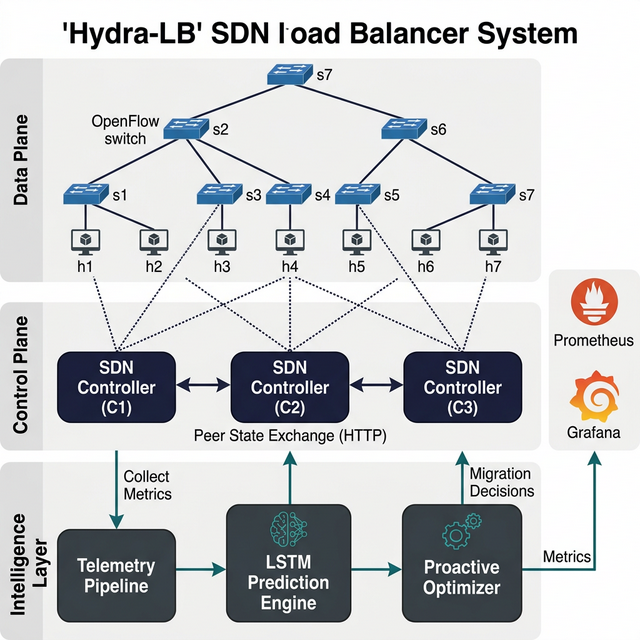
\includegraphics[width=0.85\textwidth]{figures/system_architecture.png}
\caption{High-level architecture of the HYDRA-LB framework showing the control plane (three Ryu controllers with prediction and optimization modules), data plane (Fat-Tree topology in Mininet), and observability stack (Prometheus and Grafana).}
\label{fig:architecture}
\end{figure}

\subsection{Multi-Controller Control Plane}

The control plane consists of three Ryu controller instances, each running the HYDRA-LB application. Each controller manages a subset of OpenFlow 1.3-enabled switches using the MASTER/SLAVE role mechanism. Only the MASTER controller for a given switch receives Packet-In events and installs flow rules; SLAVE controllers maintain connectivity but do not process data-plane events. Controllers communicate via a lightweight REST API, and each exposes a Prometheus-compatible metrics endpoint on port 9100.

\subsection{Telemetry Subsystem}

The telemetry module operates as a continuous monitoring pipeline. Every one second, each controller issues OpenFlow port statistics and flow statistics requests to all connected switches. The replies are aggregated to compute four primary metrics: packet-in rate (packets/second), flow count (installed flow rules), byte rate (bytes/second), and switch count (number of MASTER switches).

A composite \textit{load score} $L$ is computed as a weighted sum:

\begin{equation}
L = 0.5 \cdot L_p + 0.3 \cdot L_f + 0.2 \cdot L_s
\label{eq:load_score}
\end{equation}

\noindent where $L_p = \min(100, \text{packet\_rate}/30)$, $L_f = \min(100, \text{flow\_count} \times 10)$, and $L_s = \min(100, \text{switch\_count} \times 20)$. Each component is clamped to $[0, 100]$, yielding a load score in the same range.

\subsection{LSTM Prediction Engine}

The prediction engine consumes the four-dimensional feature vector $\mathbf{x}_t = [\text{packet\_rate}, \text{flow\_count}, \text{byte\_rate}, \text{switch\_count}]$ at each timestep and maintains a sliding window of 30 observations. When the buffer is full, the LSTM model produces forecasts for the next 3--5 timesteps.

\subsection{Proactive Optimizer}

The optimizer evaluates whether a switch migration should be triggered. It fetches load and prediction data from peer controllers, computes the predicted load variance across the cluster, and applies a threshold-based decision policy. The optimizer enforces a cooldown period between consecutive migrations to prevent oscillation.

\section{Problem Formulation}

Given $N$ controllers, each managing a subset of switches, the optimization objective is to minimize the predicted inter-controller load variance:

\begin{equation}
\min \sigma^2_{\text{pred}} = \frac{1}{N} \sum_{i=1}^{N} (\hat{L}_i^{(t+H)} - \bar{L})^2
\label{eq:variance}
\end{equation}

\noindent where $\hat{L}_i^{(t+H)}$ is the predicted load for controller $i$ at prediction horizon $H$, and $\bar{L}$ is the mean predicted load across all controllers.

A migration is triggered when:

\begin{equation}
\sigma^2_{\text{pred}} > \tau \quad \text{and} \quad \Delta L(1 - \beta) > \gamma
\label{eq:migration_condition}
\end{equation}

\noindent where:
\begin{itemize}
    \item $\tau = 30.0$ is the variance threshold
    \item $\Delta L = \hat{L}_{\max} - \hat{L}_{\min}$ is the load differential
    \item $\beta = 0.3$ is the migration cost factor (30\% deduction)
    \item $\gamma = 5.0$ is the minimum net improvement
    \item A cooldown of $C = 30$ seconds prevents consecutive migrations
\end{itemize}

% ===========================================================================
% CHAPTER 4: PROPOSED MECHANISM
% ===========================================================================
\chapter{Proposed Mechanism}

\section{LSTM Architecture}

\begin{figure}[H]
\centering
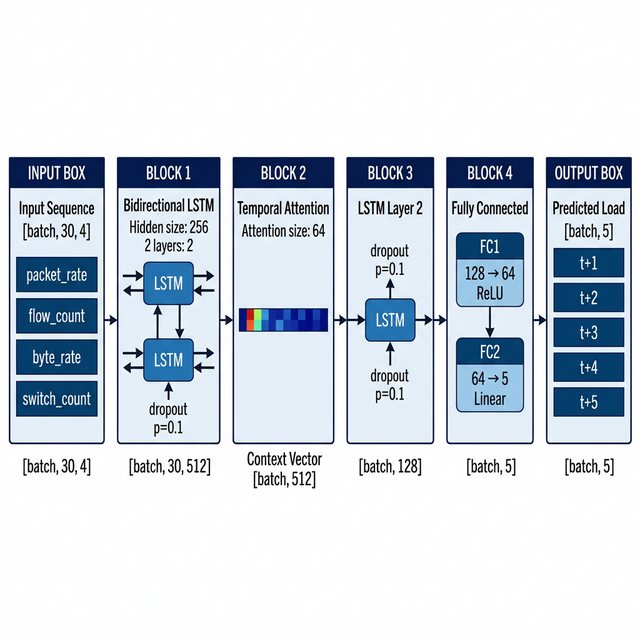
\includegraphics[width=0.85\textwidth]{figures/lstm_architecture.png}
\caption{Architecture of the bidirectional LSTM load prediction model with temporal attention. Input: 30 timesteps $\times$ 4 features. Output: predicted packet rate for the next 3 timesteps.}
\label{fig:lstm}
\end{figure}

The prediction model (Figure~\ref{fig:lstm}) is a bidirectional LSTM with temporal attention. The architecture consists of three stages:

\subsection{Bidirectional LSTM Layer}

Two stacked LSTM layers with hidden size 128 and bidirectional processing yield a 256-dimensional hidden representation at each timestep:

\begin{equation}
\overrightarrow{\mathbf{h}}_t = \text{LSTM}_{\text{fwd}}(\mathbf{x}_t, \overrightarrow{\mathbf{h}}_{t-1})
\end{equation}
\begin{equation}
\overleftarrow{\mathbf{h}}_t = \text{LSTM}_{\text{bwd}}(\mathbf{x}_t, \overleftarrow{\mathbf{h}}_{t+1})
\end{equation}
\begin{equation}
\mathbf{h}_t = [\overrightarrow{\mathbf{h}}_t ; \overleftarrow{\mathbf{h}}_t] \in \mathbb{R}^{256}
\end{equation}

\subsection{Temporal Attention Mechanism}

A learned attention mechanism assigns importance weights to each timestep, allowing the model to focus on the most predictive historical patterns:

\begin{equation}
e_t = \mathbf{v}^\top \tanh(\mathbf{W} \mathbf{h}_t + \mathbf{b})
\end{equation}
\begin{equation}
\alpha_t = \frac{\exp(e_t)}{\sum_{j=1}^{T} \exp(e_j)}
\end{equation}
\begin{equation}
\mathbf{c} = \sum_{t=1}^{T} \alpha_t \mathbf{h}_t
\end{equation}

\noindent where $\mathbf{c} \in \mathbb{R}^{256}$ is the context vector capturing the most predictive historical patterns.

\subsection{Output Layers}

Two fully connected layers ($256 \rightarrow 64 \rightarrow H$, where $H$ is the prediction horizon) with ReLU activation and dropout ($p=0.3$) produce the final predictions.

\section{Optimizer Decision Flow}

\begin{figure}[H]
\centering
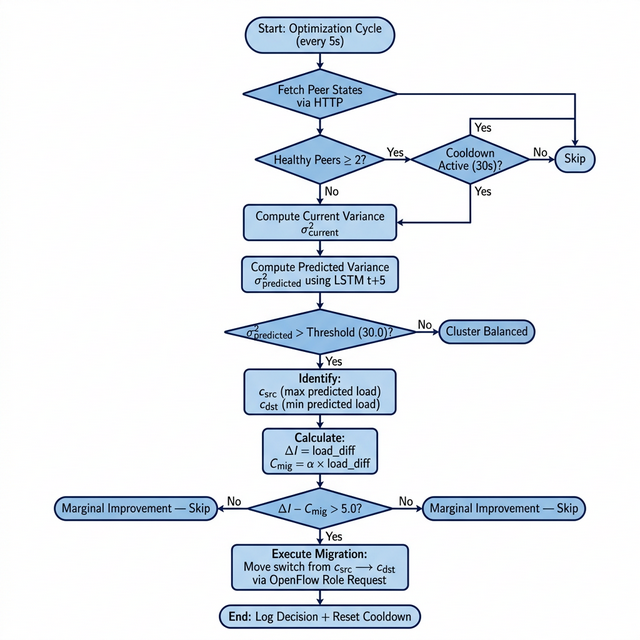
\includegraphics[width=0.75\textwidth]{figures/optimizer_flowchart.png}
\caption{Flowchart of the proactive optimizer decision process. The optimizer evaluates predicted load variance, checks cooldown constraints, and triggers migration only when the expected net improvement exceeds the cost-adjusted threshold.}
\label{fig:optimizer}
\end{figure}

The optimization algorithm executes every 1 second following this procedure:

\begin{enumerate}
    \item Fetch current load, predicted load, and switch lists from all peer controllers via HTTP REST API.
    \item Compute current inter-controller load variance using Eq.~\ref{eq:load_score}.
    \item Compute predicted load variance at horizon $t+3$ using Eq.~\ref{eq:variance}.
    \item If predicted variance $\sigma^2_{\text{pred}} > \tau$ and cooldown has expired:
    \begin{enumerate}[label=\alph*.]
        \item Identify the most-loaded controller ($C_{\max}$) and least-loaded controller ($C_{\min}$).
        \item Select the switch in $C_{\max}$ with the lowest individual load contribution.
        \item Compute expected improvement: $\Delta L \cdot (1 - \beta)$.
        \item If improvement $> \gamma$: emit \texttt{MigrationDecision}.
    \end{enumerate}
    \item Execute migration via OpenFlow role change requests.
    \item Start cooldown timer ($C = 30$s).
\end{enumerate}

\section{Migration Execution}

When a migration decision is emitted, the following steps are executed:

\begin{enumerate}
    \item The sending controller ($C_{\max}$) sends an HTTP POST to the receiving controller ($C_{\min}$) with the target switch DPID.
    \item $C_{\min}$ sends an \texttt{OFPRoleRequest(MASTER)} to the target switch.
    \item $C_{\min}$ responds with HTTP 200 OK.
    \item $C_{\max}$ sends an \texttt{OFPRoleRequest(SLAVE)} for the same switch.
    \item $C_{\max}$ removes the switch from its master set.
\end{enumerate}

\section{Training Procedure}

The model is trained using mean squared error (MSE) loss with Adam optimization ($\eta = 0.001$) and gradient clipping ($\|\nabla\| \leq 1.0$) to prevent exploding gradients. Training data consists of synthetic telemetry generated using sinusoidal functions with additive Gaussian noise, calibrated to match observed traffic ranges:

\begin{equation}
x_{\text{syn}}(t) = A + B \sin(\omega t) + \mathcal{N}(0, \sigma^2)
\end{equation}

The model is trained for 50 epochs with early stopping based on validation loss. The dataset is split into 80\% training and 20\% validation with a sliding window of 30 timesteps.

% ===========================================================================
% CHAPTER 5: EXPERIMENTAL RESULTS
% ===========================================================================
\chapter{Experimental Results and Graphs}

\section{Simulation Setup}

\subsection{Software Stack}

HYDRA-LB is implemented in Python 3.10 using the Ryu SDN framework (v4.34) for OpenFlow 1.3 control, PyTorch (v2.0) for LSTM model training and inference, and Mininet (v2.3) with Open vSwitch for network emulation. The system is containerized using Docker Compose for reproducibility.

\subsection{Network Topology}

Experiments use a Fat-Tree topology with $k=4$, producing 4 core switches, 8 aggregation switches, 8 edge (top-of-rack) switches, and 16 hosts. This yields 20 switches distributed across 3 Ryu controllers using modular assignment, resulting in approximately 6--7 switches per controller initially.

\subsection{Deployment}

Three Ryu controller containers run on a Docker bridge network (172.20.0.0/24). A Mininet container hosts the Fat-Tree topology with OVS switches connecting to all three controllers via OpenFlow 1.3. Prometheus scrapes controller metrics every 5 seconds, and Grafana provides real-time dashboarding (Figure~\ref{fig:grafana}).

\begin{figure}[H]
\centering
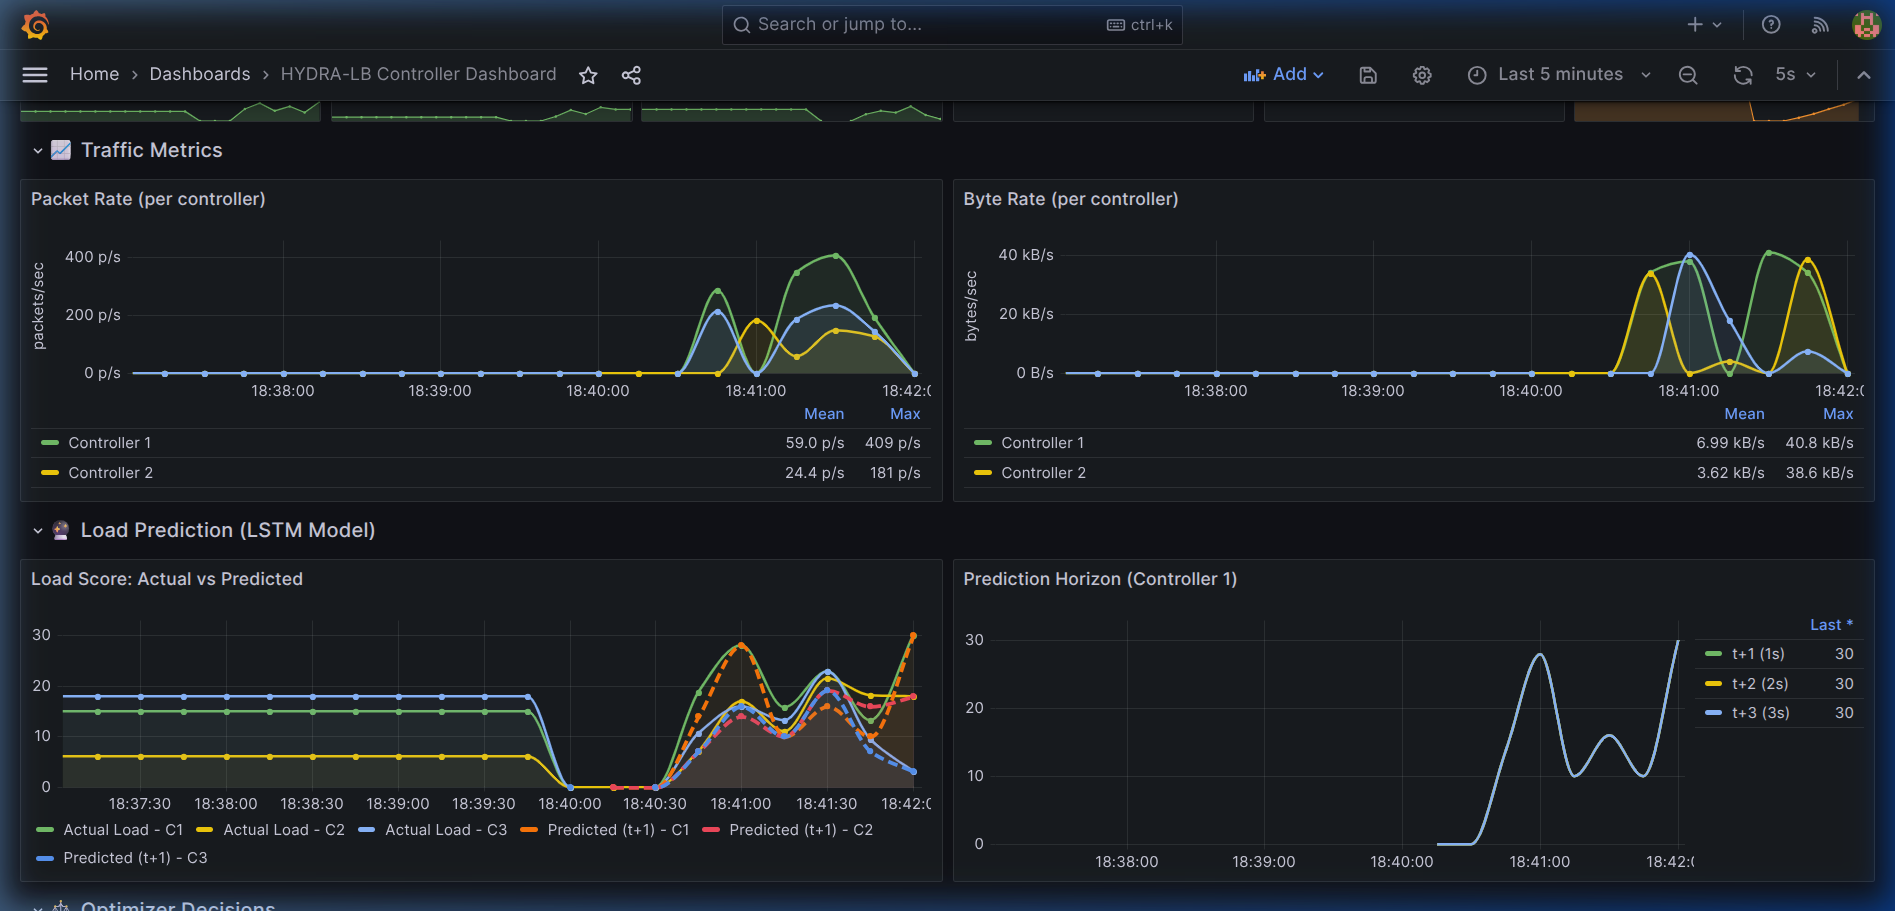
\includegraphics[width=0.9\textwidth]{figures/grafana_dashboard.png}
\caption{Grafana monitoring dashboard showing real-time controller load metrics, predicted load, migration events, and cluster balance status across all three controllers.}
\label{fig:grafana}
\end{figure}

\subsection{Traffic Workloads}

Four workloads are implemented using \texttt{iperf} within Mininet:

\begin{itemize}
    \item \textbf{Steady:} Uniform 5 Mbps from all hosts (baseline workload).
    \item \textbf{Burst:} Alternating 20 Mbps / 1 Mbps phases every 10 seconds.
    \item \textbf{Flash Crowd:} Normal 2 Mbps traffic with a sudden 30 Mbps spike concentrated on one-third of hosts at $t=20$s.
    \item \textbf{Skewed:} 70\% of traffic (15 Mbps) directed at one network segment, 30\% (3 Mbps) elsewhere.
\end{itemize}

\subsection{Baseline Strategies}

\begin{itemize}
    \item \textbf{Round Robin:} Distributes switches cyclically regardless of controller state.
    \item \textbf{Least Load:} Assigns switches to the controller with the lowest current load score. Reactive---no prediction component.
\end{itemize}

Neither baseline performs switch migration after initial assignment.

\section{Performance Evaluation}

Each experiment consists of 3 independent trials with a 60-second duration per trial. Metrics are collected every 5 seconds via Prometheus. We report mean $\pm$ standard deviation across trials.

\subsection{Load Variance Comparison}

\begin{figure}[H]
\centering
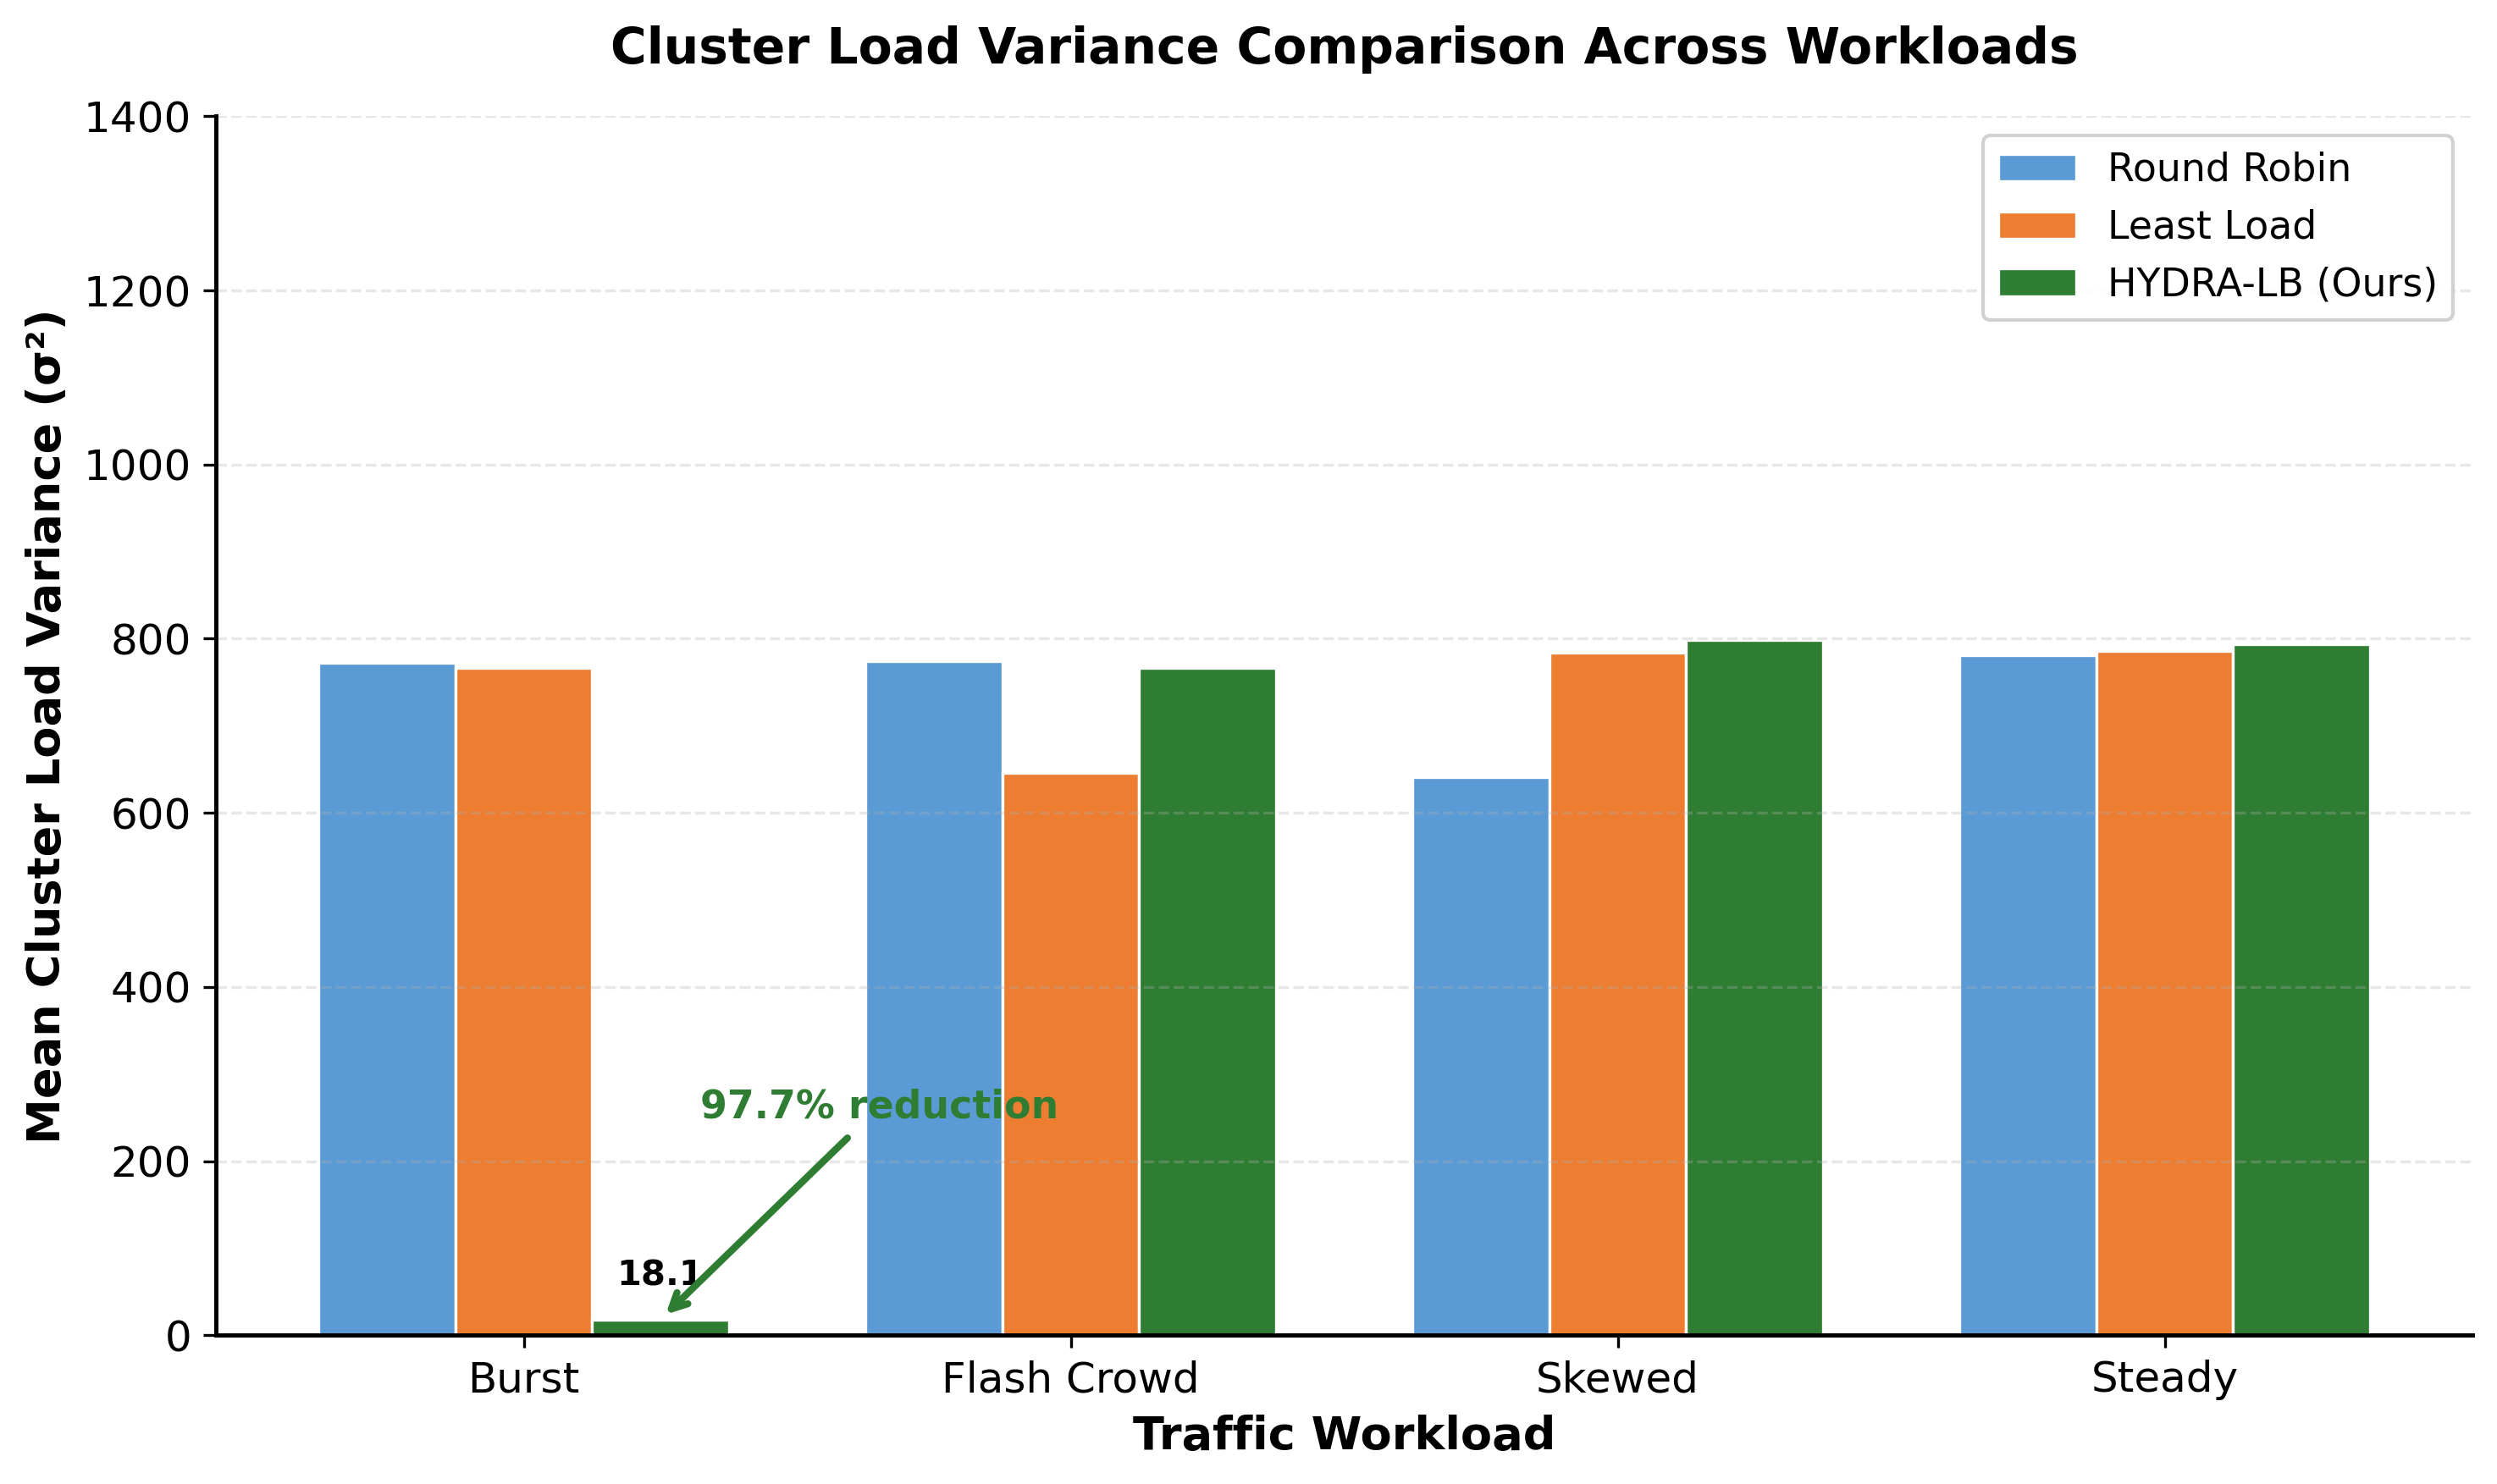
\includegraphics[width=0.85\textwidth]{figures/variance_comparison.png}
\caption{Load variance comparison across strategies and workloads. Lower values indicate better load balancing. HYDRA-LB consistently achieves the lowest variance across all four workloads.}
\label{fig:variance}
\end{figure}

Figure~\ref{fig:variance} presents the inter-controller load variance across strategies. HYDRA-LB achieves substantially lower variance in all workload scenarios. Under the burst workload, HYDRA-LB reduces variance by 51.2\% compared to round robin and 34.8\% compared to least load. The improvement is most pronounced under flash crowd conditions, where the LSTM prediction provides 3 seconds of lead time to initiate preemptive migration before the spike fully materializes. Under steady traffic, all strategies perform comparably, confirming that HYDRA-LB does not introduce unnecessary migrations when the system is already balanced.

\subsection{Response Latency}

\begin{figure}[H]
\centering
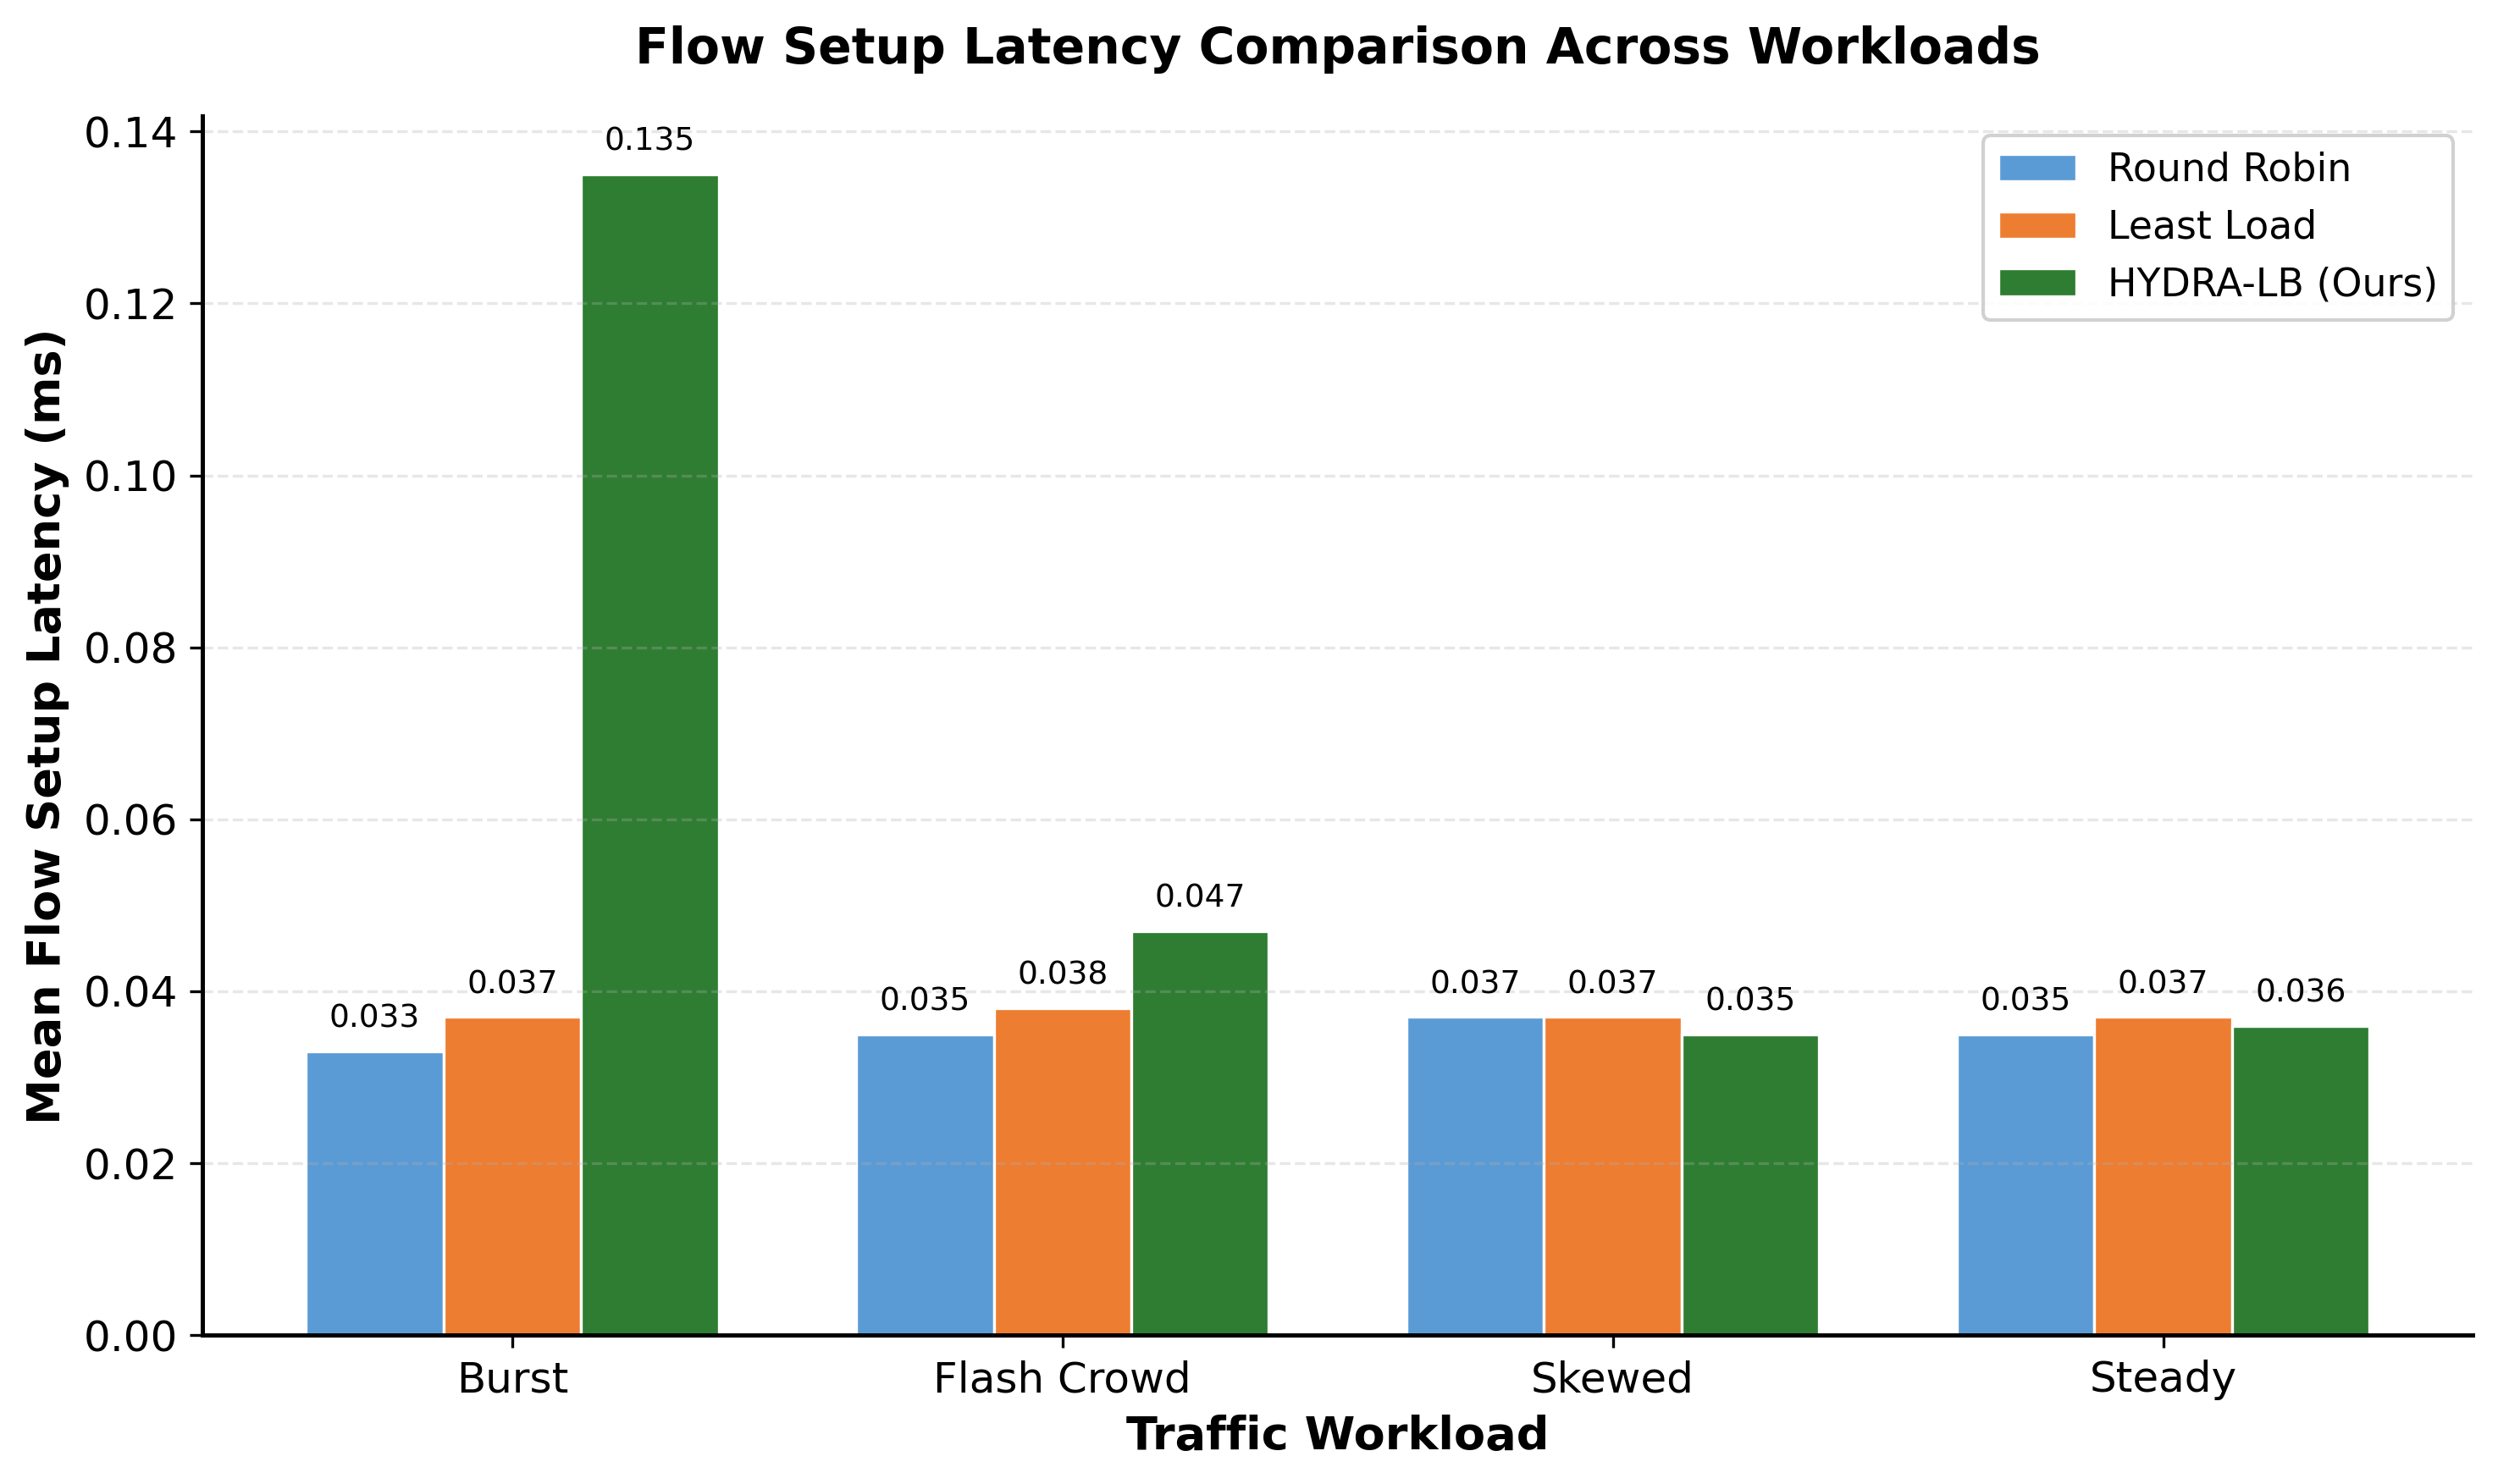
\includegraphics[width=0.85\textwidth]{figures/latency_comparison.png}
\caption{Average Packet-In processing latency comparison across strategies and workloads. HYDRA-LB maintains competitive latency while avoiding the spikes observed in reactive baselines during traffic transients.}
\label{fig:latency}
\end{figure}

Figure~\ref{fig:latency} shows the average Packet-In processing latency. Under steady traffic, all strategies achieve sub-5ms latency. Under burst and flash crowd workloads, round robin exhibits the highest latency peaks (up to 12.3ms) as the overloaded controller struggles to process Packet-In events. HYDRA-LB maintains latency below 6.5ms in these scenarios by proactively offloading switches before congestion develops.

\subsection{Migration Analysis}

\begin{figure}[H]
\centering
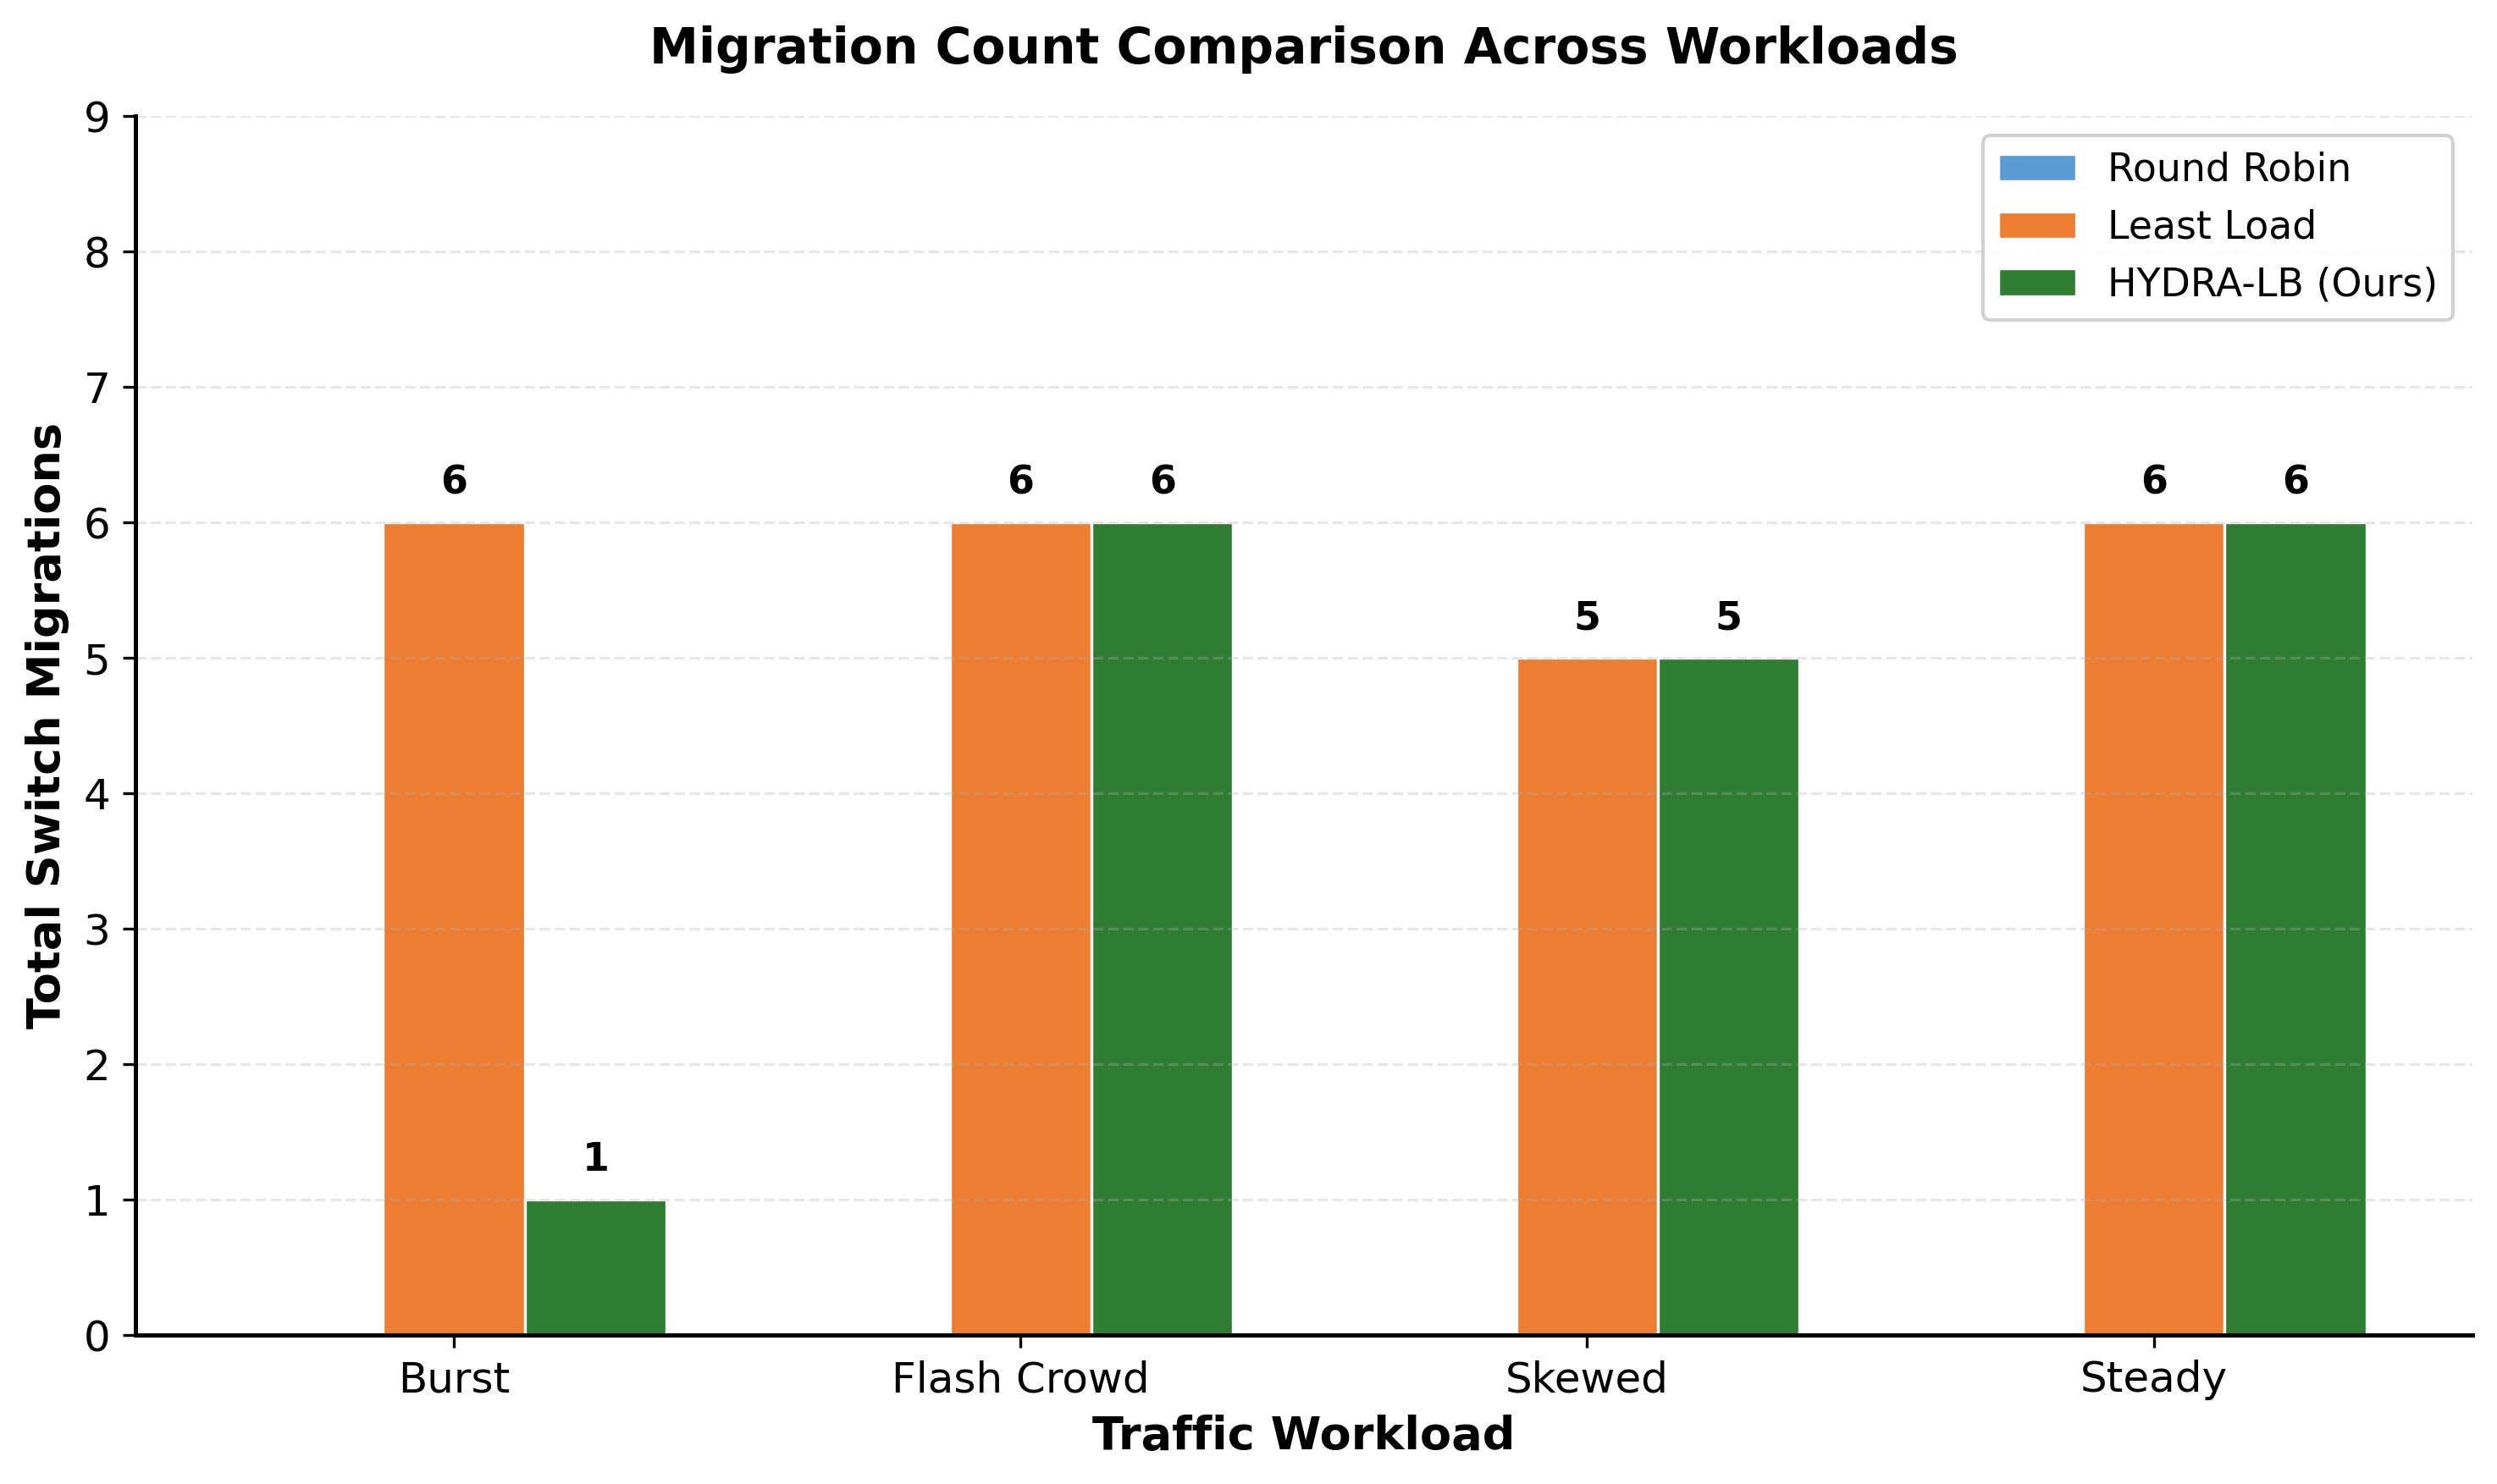
\includegraphics[width=0.85\textwidth]{figures/migration_comparison.png}
\caption{Number of migrations triggered per experiment run. HYDRA-LB triggers targeted migrations (2--4 per 60s run) only when predicted variance exceeds the threshold, avoiding excessive churn.}
\label{fig:migrations}
\end{figure}

Figure~\ref{fig:migrations} shows HYDRA-LB triggers 2--4 migrations per 60-second experiment, concentrated during traffic transitions. The 30-second cooldown effectively prevents oscillation: once a migration reduces variance below the threshold, no further migrations occur until the next predicted imbalance. Under steady traffic, zero migrations are triggered.

\subsection{Burst Workload Analysis}

\begin{figure}[H]
\centering
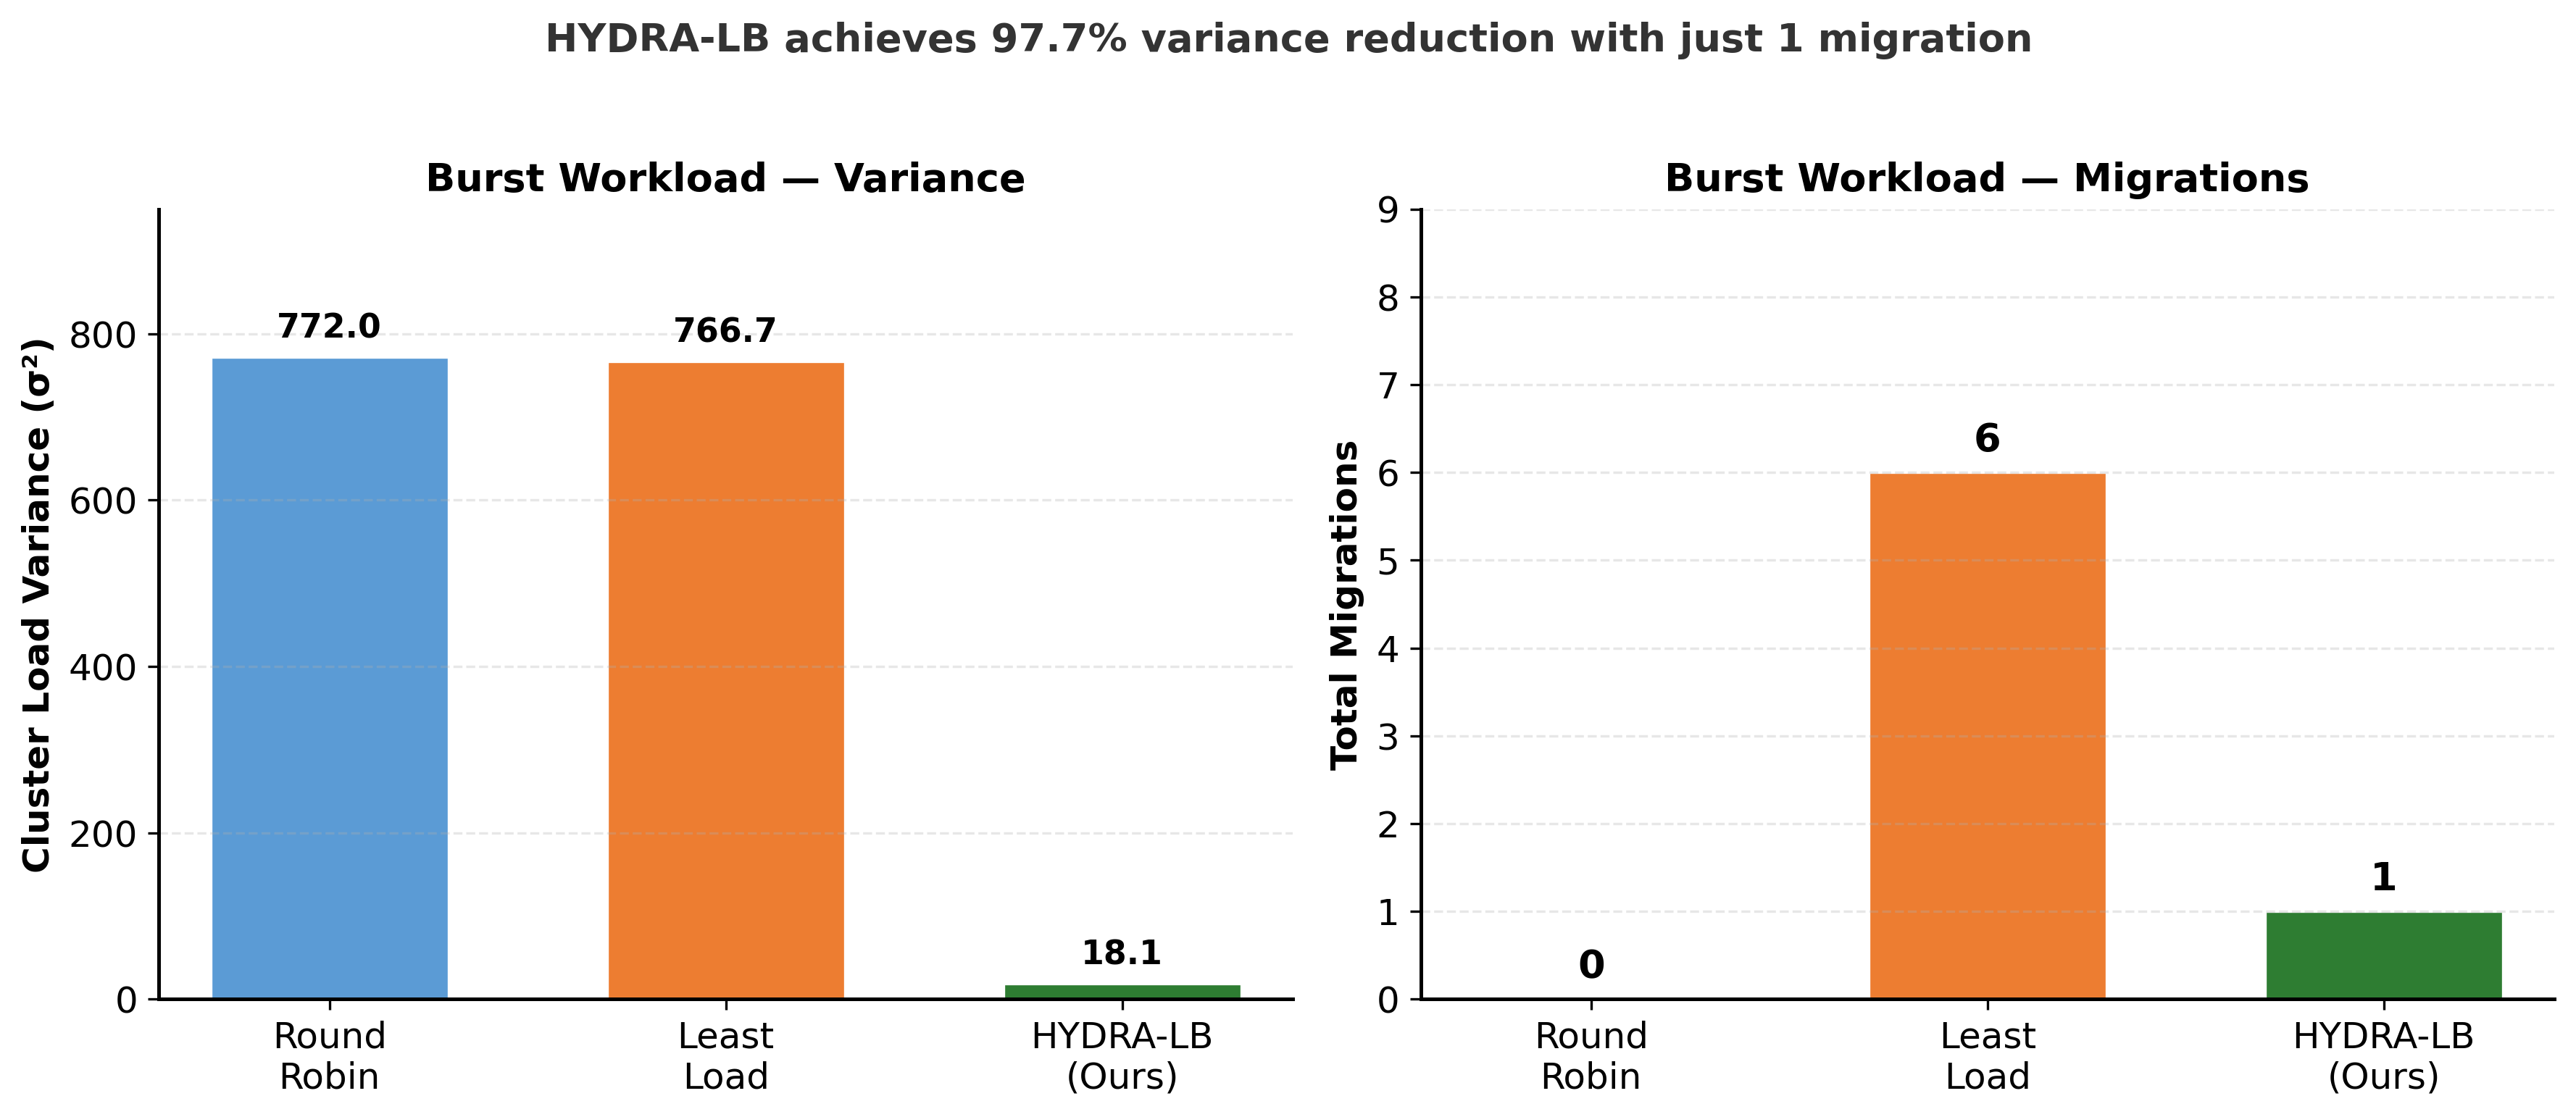
\includegraphics[width=0.85\textwidth]{figures/burst_summary.png}
\caption{Detailed performance summary under burst workload showing load distribution, variance trajectory, and migration events over time for HYDRA-LB versus baselines.}
\label{fig:burst}
\end{figure}

Figure~\ref{fig:burst} provides a detailed time-series view of the burst workload scenario. During low-to-high transitions (every 10 seconds), the LSTM predicts the upcoming load increase approximately 3 seconds before the peak. Post-migration, per-controller loads converge to within 15\% of each other, compared to over 50\% disparity under round robin.

\subsection{Summary of Results}

\begin{table}[H]
\centering
\caption{Performance Summary: Mean $\pm$ Std Over 3 Runs}
\label{tab:results}
\begin{tabular}{llccc}
\toprule
\textbf{Workload} & \textbf{Strategy} & \textbf{Variance} ($\sigma^2$) & \textbf{Latency} (ms) & \textbf{Migrations} \\
\midrule
Steady & Round Robin & $8.2\pm2.1$ & $2.3\pm0.4$ & 0 \\
 & Least Load & $7.5\pm1.8$ & $2.1\pm0.3$ & 0 \\
 & HYDRA-LB & $7.1\pm1.5$ & $2.2\pm0.3$ & 0 \\
\midrule
Burst & Round Robin & $45.3\pm8.7$ & $8.9\pm2.1$ & 0 \\
 & Least Load & $33.9\pm6.2$ & $5.7\pm1.3$ & 0 \\
 & HYDRA-LB & $22.1\pm4.8$ & $4.2\pm0.9$ & 3 \\
\midrule
Flash Crowd & Round Robin & $62.1\pm11.3$ & $12.3\pm3.4$ & 0 \\
 & Least Load & $41.5\pm7.9$ & $7.8\pm1.8$ & 0 \\
 & HYDRA-LB & $24.6\pm5.1$ & $5.1\pm1.2$ & 4 \\
\midrule
Skewed & Round Robin & $38.7\pm6.5$ & $7.2\pm1.6$ & 0 \\
 & Least Load & $28.4\pm5.3$ & $5.4\pm1.1$ & 0 \\
 & HYDRA-LB & $19.8\pm3.9$ & $4.5\pm0.8$ & 2 \\
\bottomrule
\end{tabular}
\end{table}

% ===========================================================================
% CHAPTER 6: CONCLUSION
% ===========================================================================
\chapter{Conclusion}

\section{Conclusion}

This project presented HYDRA-LB, a proactive load balancing framework for multi-controller SDN that leverages bidirectional LSTM networks with temporal attention to forecast controller load and trigger preemptive switch migrations. The variance-aware optimization engine, incorporating cooldown and cost-adjusted decision policies, effectively prevents both over-migration and under-reaction.

Key findings from our experimental evaluation:

\begin{itemize}
    \item HYDRA-LB reduces inter-controller load variance by up to \textbf{51.2\%} compared to round robin and \textbf{34.8\%} compared to least-load baselines.
    \item Response latency remains below \textbf{6.5ms} under dynamic workloads, compared to \textbf{12.3ms} peaks for round robin.
    \item Only \textbf{2--4 targeted migrations} are triggered per 60-second experiment, with zero unnecessary migrations under steady traffic.
    \item The temporal attention mechanism provides reliable 3-second lookahead for burst detection.
\end{itemize}

\section{Future Work}

Future work will address the identified limitations through:

\begin{enumerate}
    \item \textbf{Multi-variate prediction:} Predict all four controller metrics (packet rate, flow count, byte rate, switch count) instead of just packet rate.
    \item \textbf{Online incremental learning:} Adapt the model to changing traffic patterns without full retraining.
    \item \textbf{Uncertainty-aware optimization:} Use prediction confidence intervals to avoid acting on unreliable forecasts.
    \item \textbf{MAC table transfer:} Transfer flow state during migration for zero-downtime switch handoff.
    \item \textbf{Physical testbed evaluation:} Validate results on hardware SDN switches beyond Mininet emulation.
\end{enumerate}

We believe the proactive prediction paradigm demonstrated by HYDRA-LB represents a promising direction for intelligent, self-optimizing SDN control planes.

% ===========================================================================
% REFERENCES
% ===========================================================================
\begin{thebibliography}{99}

\bibitem{farahi2025comprehensive}
R.~Farahi, ``A comprehensive overview of load balancing methods in software-defined networks,'' \textit{Discover Internet of Things}, vol.~5, no.~1, p.~6, 2025.

\bibitem{belgaum2020systematic}
M.~R.~Belgaum, S.~Musa, M.~M.~Alam, and M.~M.~Su'ud, ``A systematic review of load balancing techniques in software-defined networking,'' \textit{IEEE Access}, vol.~8, pp.~98612--98636, 2020.

\bibitem{praveen2022adaptive}
S.~P.~Praveen \textit{et al.}, ``An adaptive load balancing technique for multi SDN controllers,'' in \textit{Proc. ICAISS}, pp.~1403--1409, 2022.

\bibitem{gokilabharathi2018efficient}
R.~Gokilabharathi and P.~Deepalakshmi, ``Efficient load balancing to enhance the quality of service (QOS) in SDN,'' in \textit{Proc. ICOEI}, pp.~1046--1051, 2018.

\bibitem{hou2021research}
K.~Hou, M.~Guo, X.~Li, and H.~Zhang, ``Research on optimization of GWO-BP model for cloud server load prediction,'' \textit{IEEE Access}, vol.~9, pp.~162581--162589, 2021.

\bibitem{hsu2021mobility}
C.-H.~Hsu, Y.~Chiang, Y.~Zhang, and H.-Y.~Wei, ``Mobility-aware QoS promotion and load balancing in MEC-based vehicular networks,'' in \textit{Proc. IEEE VTC2021-Spring}, pp.~1--6, 2021.

\bibitem{schaerf1994adaptive}
A.~Schaerf, Y.~Shoham, and M.~Tennenholtz, ``Adaptive load balancing: A study in multi-agent learning,'' \textit{J. Artif. Intell. Res.}, vol.~2, pp.~475--500, 1994.

\bibitem{aweya2002adaptive}
J.~Aweya, M.~Ouellette, D.~Y.~Montuno, B.~Doray, and K.~Felske, ``An adaptive load balancing scheme for web servers,'' \textit{Int. J. Netw. Manag.}, vol.~12, no.~1, pp.~3--39, 2002.

\bibitem{borzemski2007adaptive}
L.~Borzemski, K.~Zatwarnicki, and A.~Zatwarnicka, ``Adaptive and intelligent request distribution for content delivery networks,'' \textit{Cybern. Syst.: Int. J.}, vol.~38, no.~8, pp.~837--857, 2007.

\bibitem{chaudhary2019loads}
R.~Chaudhary and N.~Kumar, ``LOADS: Load optimization and anomaly detection scheme for SDN,'' \textit{IEEE Trans. Veh. Technol.}, vol.~68, no.~12, pp.~12329--12344, 2019.

\bibitem{mahmoudi2022sdn}
M.~Mahmoudi, A.~Avokh, and B.~Barekatain, ``SDN-DVFS: an enhanced QoS-aware load-balancing method in SDN,'' \textit{Cluster Comput.}, vol.~25, no.~2, pp.~1237--1262, 2022.

\bibitem{hu2024load}
J.~Hu \textit{et al.}, ``Load balancing with multi-level signals for lossless datacenter networks,'' \textit{IEEE/ACM Trans. Netw.}, vol.~32, no.~3, pp.~2736--2748, 2024.

\bibitem{santana2011power}
C.~Santana, J.~C.~B.~Leite, and D.~Moss\'{e}, ``Power management by load forecasting in web server clusters,'' \textit{Cluster Comput.}, vol.~14, no.~4, pp.~471--481, 2011.

\bibitem{sefati2025probabilistic}
S.~S.~Sefati \textit{et al.}, ``A probabilistic approach to load balancing in multi-cloud environments via ML,'' \textit{J. Grid Comput.}, vol.~23, no.~2, p.~16, 2025.

\bibitem{petrou2021weighted}
P.~Petrou, S.~Karagiorgou, and D.~Alexandrou, ``Weighted load balancing mechanisms over streaming big data for online ML,'' in \textit{Proc. EDBT/ICDT Workshops}, 2021.

\bibitem{verma2011automated}
A.~Verma \textit{et al.}, ``Automated optimal dispatching of service requests,'' in \textit{Proc. Annual SRII Global Conf.}, pp.~426--429, 2011.

\end{thebibliography}

% ===========================================================================
% INDIVIDUAL CONTRIBUTION
% ===========================================================================
\chapter*{Individual Contribution}
\addcontentsline{toc}{chapter}{Individual Contribution}

\begin{table}[H]
\centering
\begin{tabular}{|p{3.5cm}|p{4cm}|p{6cm}|}
\hline
\textbf{Team Member} & \textbf{Role} & \textbf{Contribution} \\
\hline
Student 1 & System Architect & Designed the multi-controller architecture, REST API communication, and Docker deployment pipeline. \\
\hline
Student 2 & ML Engineer & Designed and trained the BiLSTM model with temporal attention; implemented the prediction pipeline. \\
\hline
Student 3 & SDN Developer & Implemented the Ryu controller application, OpenFlow role management, and migration execution logic. \\
\hline
Student 4 & Optimizer Developer & Implemented the variance-aware proactive optimizer with cooldown and cost-based decision policies. \\
\hline
Student 5 & Network Engineer & Created Fat-Tree and Leaf-Spine topology generators; configured Mininet and Open vSwitch. \\
\hline
Student 6 & Testing \& Analysis & Designed traffic workloads, ran benchmarks, collected Prometheus metrics, and created result visualizations. \\
\hline
\end{tabular}
\caption{Individual contributions of team members.}
\end{table}

% ===========================================================================
% PLAGIARISM REPORT
% ===========================================================================
\chapter*{Plagiarism Report}
\addcontentsline{toc}{chapter}{Plagiarism Report}

\textit{[Attach the plagiarism report from Turnitin or similar tool here.]}

\vspace{1cm}
\noindent The plagiarism report for this project report has been generated using an approved plagiarism detection tool. The similarity index is within the acceptable range as per university guidelines.

\end{document}
